% -*- coding: UTF-8 -*-
% vim: autoindent expandtab tabstop=4 sw=4 sts=4 filetype=tex
% vim: spelllang=de spell
% chktex-file 27 - disable warning about missing include files

\section{Logische Architektur}
\label{sec:logical-architecture}

Die logische Architektur zeigt das Gesamtbild der Software-Klassen in Form von
Paketen (bzw. Namespaces), Subsystemen und Layern~\cite{larman_applying_2004}.
Bei Layern handelt es sich um eine grobe Gruppierung von Klassen, Paketen oder
Subsystemen, welche zusammenhängen~\cite{larman_applying_2004}.

\subsection{Player}
\label{subsec:package-diagram:player}

\begin{figure}[H]
    \centering
    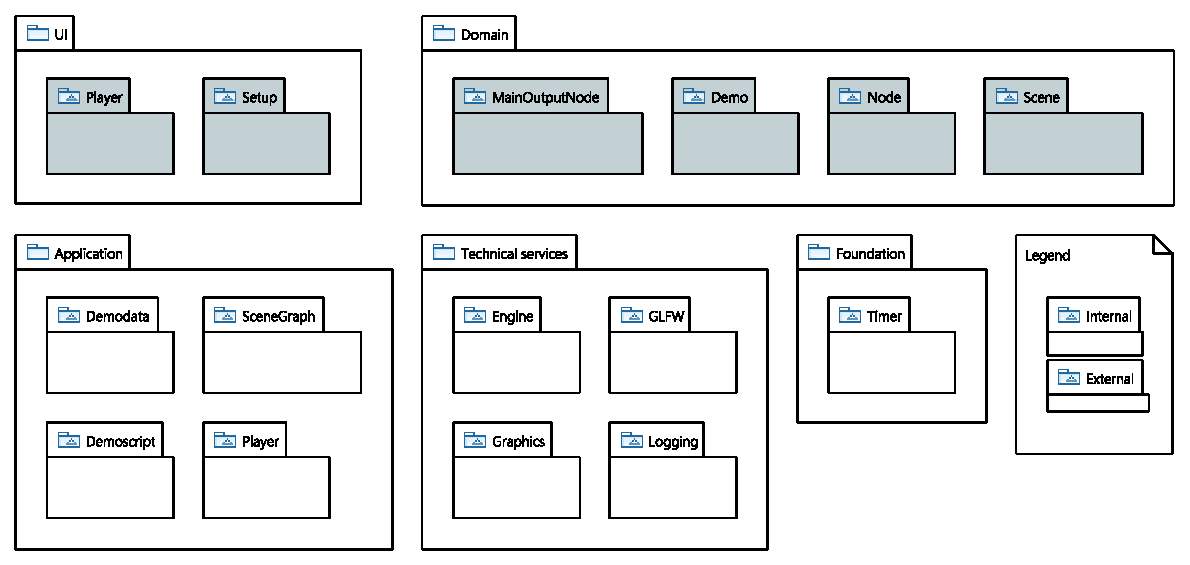
\includegraphics[width=0.7\textwidth]{img/player_package_diagram.pdf}
    \caption{Paket-Diagramm der
        Player-Applikation\protect\footnotemark}\label{fig:package-diagram:player}
\end{figure}
\footnotetext{Eigene Darstellung mittels Papyrus.}

\todo[inline]{Describe player package diagram.}

\subsection{Editor}
\label{subsec:package-diagram:editor}

\begin{figure}[H]
    \centering
    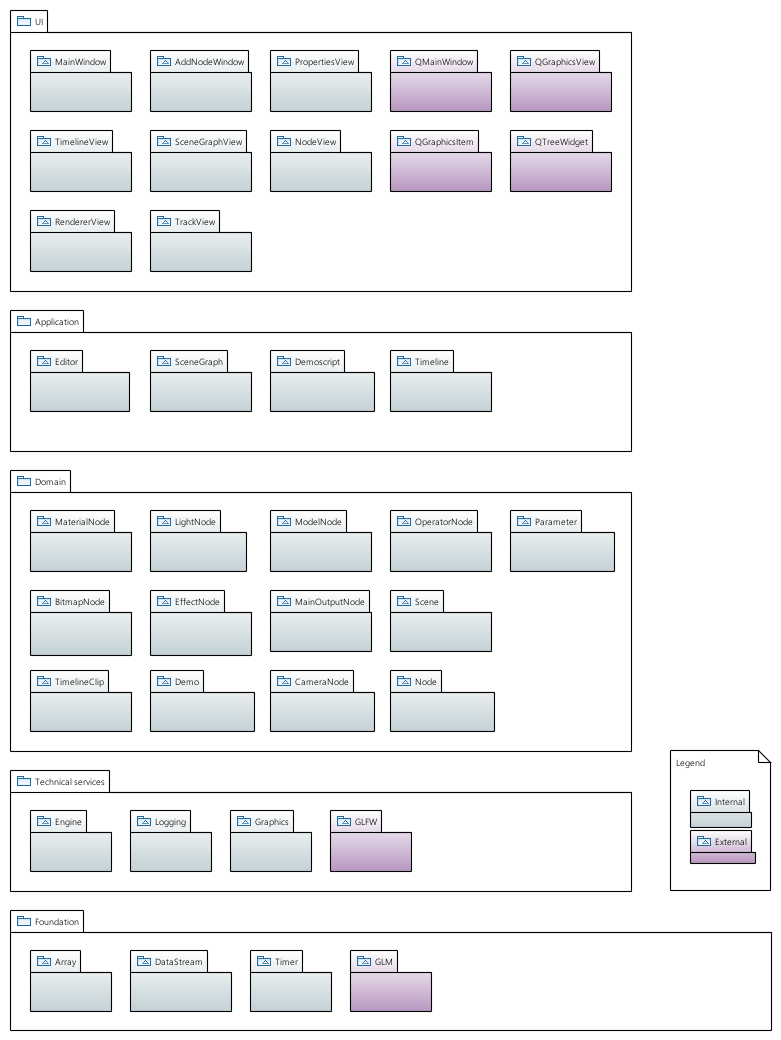
\includegraphics[width=0.9\textwidth]{img/editor_package_diagram.pdf}
    \caption{Paket-Diagramm der
        Editor-Applikation\protect\footnotemark}\label{fig:package-diagram:editor}
\end{figure}
\footnotetext{Eigene Darstellung mittels Papyrus.}

\todo[inline]{Describe editor package diagram.}
